\begin{tikzpicture}
%\draw (-0.5,-1.5) -- (12,-1.5);
    \draw (-0.5,1)node[left,font=\tiny] {$y=+1~~~~$} -- (11.8,1);
    \draw (-0.5,-1)node[left,font=\tiny] {$y=-1~~~~$} -- (11.8,-1);
    \draw (-0.5,-0.33)node[left,font=\tiny] {$y=-0.33$} -- (11.8,-0.33); 
    \draw (-0.5,0.33)node[left,font=\tiny] {$y=+0.33$} -- (11.8,0.33); 
    \foreach \x in {0,0.25,...,12}
    {
    	\draw (\x*4,-1.5)node [below,font=\tiny,] {\x} -- (\x*4,1.5) ;
    }
    \draw[ultra thick, red] (0,0) sin (1,1);
    \draw[ultra thick, blue] (1,1) cos (2,0);
    \draw[ultra thick, red] (2,0) sin (3,-1);
    \draw[ultra thick, blue] (3,-1) cos (4,0);
    \draw[ultra thick, red] (4,0)  sin (5,1);
    \draw[ultra thick, blue] (5,1) cos (6,0);
    \draw[ultra thick, red] (6,0) sin (7,-1);
    \draw[ultra thick, blue] (7,-1) cos (8,0); 
\end{tikzpicture}